% !TeX root = ../tjuthesis-example.tex

\section{排版示例}

这一章中我们给出一些排版示例, 以便一些对\LaTeX 不熟悉的同学来学习参考.
% TODO: 列举

\subsection{插图}

我们先来整理一下手册对插图的要求. 手册第十九页及第二十页的撰写规范中提到:
\begin{quote}
  毕业设计 (论文) 的插图 (此处插图系指正文中的插图) 必须精心制作, 线条粗细要合适, 图面要整洁美观. 每幅插图应有图序和图题, 图序和图题应放在图位下方居中处. 图序, 图题采用宋体小5号. 图应在描图纸或在白纸上用墨线绘成, 也可以用计算机绘图. 插图上下均应空一行.
\end{quote}
手册第五十二页的参考例文中提到:
\begin{quote}
  图居中, 上下与正文之间各空一行.
  图中文字: 小五, 宋体 (英文 Times New Roman), 行距1倍, 段前0行, 段后0行.
  插图应有图序和图题, 全文插图以章分组编序号, 图序必须连续, 不得重复或跳缺. 如图4.1表示第四章的第一幅图.
  图题: 小五, 宋体 (英文 Times New Roman), 居中置于图下方, 行距18磅, 段前0行, 段后0行.
\end{quote}

现在我们应该来说一下应该如何排版插图. 我们在文档类中已经引用了 \pckg{graphicx} 宏包\footnotemark 和 \pckg{caption} 宏包, 并做好了图序图题的格式定制, 要注意图序图题之间空一格, 无其余分隔符. 我们利用 \verb|\captionsetup| 宏配置了全局的 \verb|font|, \verb|labelsep| 和 \verb|skip| 选项, 并配置了 \verb|figure| 环境的 \verb|position| 选项. 文档类中也引用了 \pckg{chngcntr} 宏包, 用此设置了 \verb|figure| 环境的计数器.

绘制插图的方法, 其中参数的含义以及浮动体的介绍可以参考 \pckg{latex2e} 的文档, 我们就不在这里详细展开了. 我们拿手册中的插图来作为示例. 需要注意的是 \verb|figure| 环境的参数是我个人的喜好, 如果想要强制浮动体在当前位置输出的话可以参考 \pckg{float} 宏包. 还需要注意 \verb|\caption| 宏应该写在 \verb|\includegraphics| 宏的下方, 如果需要用 \verb|\label| 宏则应放在 \verb|\caption| 宏之后. 不建议用户在这里设置插图的大小或者缩放, 这件事情应当在绘制插图的时候就做好, 否则难以保证对插图内文字的格式要求. \ref{fig:xlccd-single} 是单张图的一个示例.
\footnotetext{好像 \pckg{graphicx} 包提供的接口没有被用到?}

\begin{figure}[htb]
  \centering
  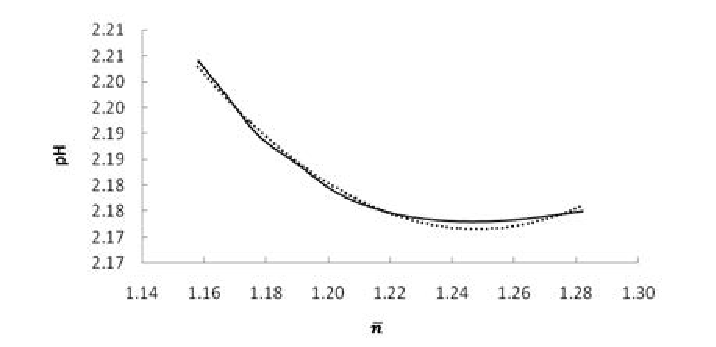
\includegraphics{figures/oxalic-acid-n-geq-1.15.pdf}
  \caption{乙二酸$\overline{n}\geq 1.15$数据段曲线及其拟合曲线 (实线--实际曲线, 虚线--拟合曲线) 乙二酸$\overline{n}\geq 1.15$数据段曲线及其拟合曲线 (实线--实际曲线, 虚线--拟合曲线) 乙二酸$\overline{n}\geq 1.15$数据段曲线及其拟合曲线 (实线--实际曲线, 虚线--拟合曲线)}\label{fig:xlccd-single}
\end{figure}

在排版过程中我们会遇到多列子图的情况, 我们在文档类中已经引用了 \pckg{subcaption} 宏包, 并做好了子图的图序和图题的格式定制. 我们利用 \verb|subfigure| 环境来排版子图, 它的第一个可选参数 \verb|<outer-pos>| 表示子图整个盒子的垂直位置, 可选项为 ``c", ``t", ``b", ``T", ``B", 可以参考 \pckg{latex2e} 文档中关于 \verb|minipage| 环境及参数的介绍以及 \pckg{subcaption} 宏包文档的相关内容来明白这些参数以及其它可选参数的含义. \verb|subfigure| 环境的必选参数表示这张子图及图题所占的宽度, 它不会帮你缩放插图, 但会决定图题所占的宽度, 注意\verb|\linewidth| 表示去除边界之后的页面宽度, 一行之中所有子图的宽度之和不要超过这个宽度. 下面的例子中要注意仅在子图要换行的时候添加空行, 还要注意 \verb|\hfil| 宏保证了这些子图之间以及与页边的水平间距合适, 关于 \verb|\hfil| 宏可以参考\href{https://tex.stackexchange.com/a/528921/184559}{这个 TeX.SE 中的回答}. 每张子图可以分别加上标签, 比如\ref{fig:tju}是我们多行多列子图的示例, 而\ref{fig:tjusub1}是其中第一张子图. 关于引用时标签输出格式的设定, 我们准备放到以后再研究.

\begin{figure}[htb]
  \hfil
  \begin{subfigure}[b]{0.4\linewidth}
    \centering
    
\includegraphics{tongji-name-bacholar.jpg}
    \caption{乙二酸$\overline{n}\geq 1.15$数据段曲线及其拟合曲线 (实线--实际曲线, 虚线--拟合曲线)}\label{fig:tjusub1}
  \end{subfigure}
  \hfil
  \begin{subfigure}[b]{0.4\linewidth}
    \centering
    
\includegraphics{tongji-name-bacholar.jpg}
    \caption{乙二酸$\overline{n}\geq 1.15$数据段曲线及其拟合曲线 (实线--实际曲线, 虚线--拟合曲线)}
  \end{subfigure}
  \hfil

  \hfil
  \begin{subfigure}[b]{0.4\linewidth}
    \centering
    
\includegraphics{tongji-name-bacholar.jpg}
    \caption{乙二酸$\overline{n}\geq 1.15$数据段曲线及其拟合曲线 (实线--实际曲线, 虚线--拟合曲线)}
  \end{subfigure}
  \hfil
  \begin{subfigure}[b]{0.4\linewidth}
    \centering
    
\includegraphics{tongji-name-bacholar.jpg}
    \caption{乙二酸$\overline{n}\geq 1.15$数据段曲线及其拟合曲线 (实线--实际曲线, 虚线--拟合曲线)}
  \end{subfigure}
  \hfil
  \caption{乙二酸$\overline{n}\geq 1.15$数据段曲线及其拟合曲线 (实线--实际曲线, 虚线--拟合曲线)}\label{fig:tju}
\end{figure}

\zhlipsum[1]

\subsection{表格}

我们先来整理一下手册对插图的要求. 手册第十九页的撰写规范中提到:
\begin{quote}
  每个表格应有表序和表题, 表序和表题应写在表格上方正中, 表序后空一格书写表题. 表序, 表题采用宋体小5号. 表格允许下页接写, 表题可省略, 表头应重复写, 并在右上方注明 ``{\songti 续表XX}". 表格上下均应空一行.
\end{quote}
手册第五十一页及第五十二页的参考例文中提到:
\begin{quote}
  表格上下与正文之间各空一行;
  采用三线表, 两端与页面对齐;
  表中文字: 小五, 宋体 (英文 Times New Roman), 行距 18 磅, 段前 0 行, 段后 0 行.

  表序写在表题左方不加标点, 空一格写表题, 表题末尾不加标点, 表格逐章编序, 表序必须连续, 如表 4.4 表示第四章的第四个表. 表题: 小五, 宋体 (英文 Times New Roman), 居中置于表上方, 行距 18 磅, 段前 0 行, 段后 0 行.

  若表格分页, 则该表第 2 页的表题省略, 但表头应重写, 并在表右上方加注 ``续表 X.X";
  ``续表 X.X" 的格式: 小五, 宋体 (英文 Times New Roman), 行距 18 磅, 段前 0 行, 段后 0 行, 右空 2 格.
\end{quote}

现在我们应该来说一下应该如何排版表格. 类似于插图的情况, 我们做好了表序表题的格式定制, 设置好了 \verb|table| 环境的计数器. 我们利用 \verb|\captionsetup| 宏配置了 \verb|table| 环境的 \verb|position| 选项. 文档类中还引用了 \pckg{array} 宏包和 \pckg{booktabs} 宏包, 用来改良 \verb|tabular| 环境并制作漂亮的三线表.

类似于插图, 正文中的表格一般也以浮动体的形式出现. 绘制表格的方法, 其中参数的含义以及浮动体的介绍可以参考 \pckg{latex2e} 的文档, 我们就不在这里详细展开了. 需要注意的是 \verb|\caption| 宏应该写在 \verb|\includegraphics| 宏的上方, 同样如果需要用 \verb|\label| 宏则应放在 \verb|\caption| 宏之后. 还需要注意的是表格内各类元素的字体需要统一, 比如不能有的数字用数学字体, 有的数字用文字字体. \emph{在排版过程中我们发现手册第 50 页的参考例文中的表格, 似乎其上方的正文空了两行.} 我们并不准备对此进行模仿.

手册要求表格的两端与页面对齐, 关于这个排版需求我知道两种方法, 可以参考\href{https://tex.stackexchange.com/questions/10535}{这个 TeX.SE 问题}中的\href{https://tex.stackexchange.com/a/56552}{这个回答}和\href{https://tex.stackexchange.com/a/10540}{这个回答}. 两种方法的主要区别在于, 第一种方法没有改变每一列的宽度, 而是通过增加列之间的距离来实现表格宽度的增加, 第一种方法不需要引用额外的宏包. 第二种方法通过增加每一列的宽度来实现表格宽度的增加, 需要引用 \pckg{tabularx} 宏包. 我们并没有在文档类中引用 \pckg{tabularx} 宏包, 用户若有需要可以自行引用. 文档类中为了设置表格中文字的格式在 \verb|tabular*| 环境和 \verb|tabularx| 环境之前添加了设置字体大小和行距的命令.

\ref{tab:xlccd}展示了如何用第一种方法进行不跨页表格的排版, 跨页表格的排版我们之后再做. 之后我们还会考虑使用 \pckg{pgfplotstable} 宏包进行表格的排版, 因为那样可以省去我们在表格的每一个位置都加上数学环境的麻烦.

\begin{table}[htb]
  \caption{草酸的部分数据列表}\label{tab:xlccd}
  \begin{tabular*}{\textwidth}{c @{\extracolsep{\fill}} cccc}
    \toprule
    $V\!\unit{mL}$ & $E\unit{mV}$ & $\mathrm{pH}$ & $[\hydrgenn]\unit{mod\cdot L^{-1}}$ & $\overline{n}$\\
    \midrule
    $\dotsb$ & $\dotsb$ & $\dotsb$ & $\dotsb$ & $\dotsb$\\
    \\
    $1.00$ & $2.62\times 10^2$ & $2.22$ & $6.07\times 10^{-3}$ & $1.14$\\
    $1.50$ & $2.60\times 10^2$ & $2.27$ & $5.42\times 10^{-3}$ & $1.10$\\
    \\
    $\dotsb$ & $\dotsb$ & $\dotsb$ & $\dotsb$ & $\dotsb$\\
    \bottomrule
  \end{tabular*}
\end{table}

\zhlipsum[1]

\subsection{代码}

有时论文中需要附上代码, 一般来说代码高亮可以采用 \pckg{listing} 包或者 \pckg{minted} 包, 在文档类中这两个包都没有引用, 用户可以选用自己习惯的方式. 在这里推荐使用 \pckg{minted} 包, 文档类中也对此进行了配置, 使得宏包的标准接口就可以满足大部分排版要求.

使用 \pckg{minted} 包进行代码高亮需要首先安装 \href{https://wiki.python.org/moin/BeginnersGuide/Download}{Python}, 以及 Python 中的 \href{https://pygments.org/download/}{Pygments} 包, 并在 \LaTeX 编译时添加 \verb|--shell-escape| 选项以启用外部程序.

安装完成过后, \pckg{minted} 的使用方法就比较简单了, 只需要
\begin{verbatim}
  \begin{listing}
    \caption{<caption>}\label{<label>}
    \inputminted{<language>}{<filename>}
  \end{listing}
\end{verbatim}
就可以了, 跨页代码块也可以如此排版. 可以进行高亮的语言可以通过在命令行中输入
\begin{verbatim}
  pygmentize -L lexers
\end{verbatim}
进行查询. 如果用户对文档类中配置的代码块样式不满意, 可以使用 \verb|\setminted| 命令自行修改, 具体参考 \pckg{minted} 宏包的文档. \ref{code:JD-iter} 是一个较短 Matlab 代码块的例子, 而 \ref{code:NN-init} 是一个较长 Python 代码块的例子, 放入附录.

\begin{listing}
  \caption{Jacobi-Davidson 迭代法}\label{code:JD-iter}
  \inputminted{matlab}{codes/jacobi_davidson.m}
\end{listing}

要注意文档类中引用了 \pckg{mdframed} 包. 还要注意因为通常代码块中会含有大量的字符, 使用 MikTeX 发行版的用户可能会得到 TeX 容量超出限制的报错, 此时需要先查看 log 找到是哪些容量不够了, 然后按照\href{https://tex.stackexchange.com/a/548335/}{这个回答}中的方法来扩充可用容量. 如果代码块里有过长的行可能无法排版, 建议不要出现超过 80 个字符的行. 如果用户还遇到了其它错误, 可以先考虑删除所有的临时文件以及 \pckg{minted} 生成的缓存文件夹 (以 ``\_minted" 打头) 再重新进行编译.
